\chapter{Emotion Recognition}
% Afsnit x.1 - Introduktion, da vi har dataen, kan vi lave modellen
Now that that the dataset of GSR and PPG data is available, it is possible to train a emotion recognition model. To this end, the tensorflow framework will be used to design and train the model. The model that is used for emotion detection is a CNN netowrk which is inspired from \cite{CNNEmotionDetection}. This model consists of an input layer that takes a sample of PPG data and a sample of GST data. The hidden layers of the model, consists of 2 convolution layers, with a filter size of 32 and 64 respectively. Furthermore, both convolution layers uses a kernel size of 3x1, a stride of 1 and a ReLu activation function. Each layer is also followed by a max pooling layer, with a pool size of 2. At the end of the network, a dropout layer is used, with a dropout of 0.5, followed by a dense that serves as the output layer. The dense layer uses a filter of 4, which symbolizes low arousal, high arousal, low valance and high valance. In order to ensure that these values is a probability that sums to 1, the softmax acitvation layer is used.  

%Afsnit x.3 - Hardware


%Afsnit x.4 - Epoch, batch-size, training time

%Afsnit x.5 - Results

\begin{figure}[H]
    \centering
    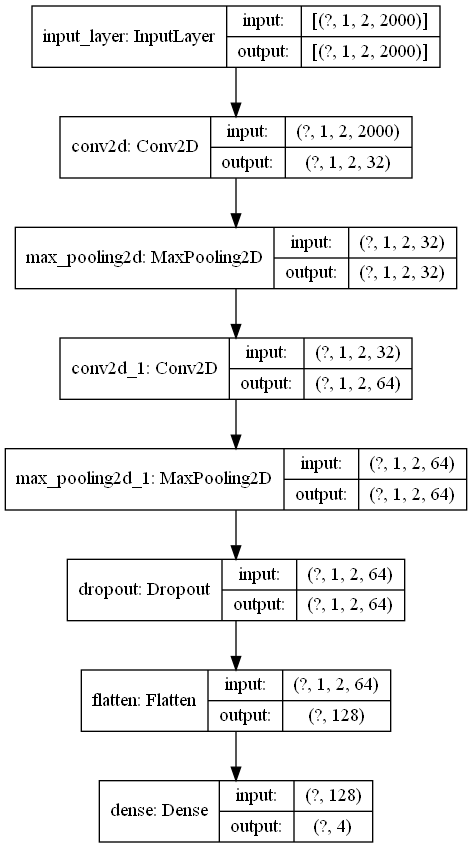
\includegraphics[width=0.8\textwidth]{figures/Emotion_Detetion_Model.png}
    \caption{Emotion Detection Model}
    \label{fig:EmotionDetectionModel}
\end{figure}